\documentclass{article}
 

 
\usepackage[margin=1in]{geometry} 
\usepackage{amsmath,amsthm,amssymb}
 \usepackage{graphicx}
 \usepackage{enumerate}
 
 
\newcommand{\N}{\mathbb{N}}
\newcommand{\Z}{\mathbb{Z}}

\newcommand\numberthis{\addtocounter{equation}{1}\tag{\theequation}}

\def\R{\mathbb{R}}
\def\Zp{\mathbb{Z}^+}

\def\a{\alpha}
\def\b{\beta}
\def\c{\gamma}

 
\begin{document}
 
% --------------------------------------------------------------
%                         Start here
% --------------------------------------------------------------
 
 
%%%%%%%%%%%%%%%%%%%%%%%%%%%%%%%%%
% TITLE PAGE
%%%%%%%%%%%%%%%%%%%%%%%%%%%%%%%%% 
\title{
    \textmd{\Huge{Midterm A1}}\\
    \textmd{\huge{Section 4}}
}


\maketitle

Consider the set of points $(-2, 2)$, $(0, 1)$ and $(2, 2)$ and the interpolating polynomial $f(x)$, which is a $2^\text{nd}$ degree polynomial that passes through those points. \\

\textbf{Problem 1} [5pt]: If $f(x)$ is written as $\a x^2 + \b x + \c$, write down the linear system to be solved to obtain $\a$, $\b$ and $\c$. \\

Before anything, I do a quick sketch to see what's going on. \hspace*{3cm}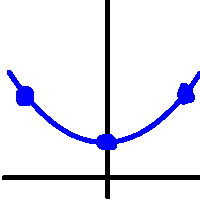
\includegraphics[scale=0.5]{thumbSketch}\\

Then I write down my given information.

\[
f(x) = \a x^2 + \b x + \c 
\]

Then I realize that this question is asking me to write down a system of equations, not find the scalar values $\a$, $\b$ and $\c$. Make note that these equations must be \textit{linear}. What are three equations I can write with the given information? There's only one thing I can do, really. I have three points and an equation. So I'm just going to plug each given $x$ value in and equate that with its $y$ value like this.

\begin{align*}
y_1 &= f(x_1) = \a x_1^2 + \b x_1 + \c \\
y_2 &= f(x_2) = \a x_2^2 + \b x_2 + \c \numberthis \\
y_3 &= f(x_3) = \a x_3^2 + \b x_3 + \c  \\
\end{align*}

Knowing that I'm looking for a linear system of equations, and knowing that \textit{linear system of equations} is a fancy way of saying \textit{matrix equation}, I'm going to rewrite it like this when I substitute the $(x_i, y_i)$'s back in. 

\begin{align*}
 \a (-2)^2 - \b 2 + \c &= 2 \\
 \a 0^2 + \b 0 + \c &= 1 \numberthis \\
 \a 2^2 + \b 2 + \c &= 2 \\
\end{align*}

If you weren't on facespace while the AMATH 301 lectures were playing dimly in the background, you'll probably recognize that (2) can be rewritten in fancy form like this.

\[
\begin{pmatrix} (-2)^2 & -2 & 1 \\ 0^2 & 0 & 1 \\ 2^2 & 2 & 1\\ \end{pmatrix}
\begin{pmatrix} \a \\ \b \\ \c \\ \end{pmatrix} = 
\begin{pmatrix} 2 \\ 1 \\ 2 \\ \end{pmatrix} \numberthis
\] 

And if you're really on your game, you can do this.

\[
\begin{pmatrix} 4 & -2 & 1 \\ 0 & 0 & 1 \\ 4 & 2 & 1\\ \end{pmatrix}
\begin{pmatrix} \a \\ \b \\ \c \\ \end{pmatrix} = 
\begin{pmatrix} 2 \\ 1 \\ 2 \\ \end{pmatrix} \numberthis
\] 

I awarded 5 points if you proved to me that you knew what you were doing. If you wrote down (2), (3), or (4), then you nailed it. Note that something along these lines would be a perfectly good answer

\begin{align*}
y_1 &=  \a x_1^2 + \b x_1 + \c \\
y_2 &=  \a x_2^2 + \b x_2 + \c \\
y_3 &=  \a x_3^2 + \b x_3 + \c  \\
\end{align*}
\[
\text{where} \;\; \begin{pmatrix} x_1 \\ x_2 \\ x_3 \end{pmatrix} = \begin{pmatrix} -2 \\ 0 \\ 2 \end{pmatrix} \;\; \text{and} \;\; \begin{pmatrix} y_1 \\ y_2 \\ y_3 \end{pmatrix} = \begin{pmatrix} 2 \\ 1 \\ 2 \end{pmatrix}
\] \\

because it would \textit{prove to me} that you know what you're doing. I'm surprised nobody tried that. \\

\textbf{Problem 2} [10pt]: The system above can be row-reduced to the following system:

\[
\begin{pmatrix} 4 & -2 & 1 \\ 0 & 4 & 0 \\ 0 & 0 & 1 \end{pmatrix} \begin{pmatrix} \a \\ \b \\ \c \end{pmatrix} = \begin{pmatrix} 2 \\ 0 \\ 1 \end{pmatrix}
\]

Solve this system for $\a$, $\b$, and $\c$.\\

When all else fails, just play with the given information. Get it into a new form which




\end{document}











































